\chapter{Rétention et Replay}

\section{Pourquoi la Rétention est Essentielle}

La \textbf{rétention des événements} est le concept fondamental qui fait de Kappa une architecture viable. Sans rétention, impossible de faire du replay. Sans replay, pas de Kappa.

\begin{infobox}
    \centering
    \vspace{0.3cm}
    {\large La \textbf{rétention} est la durée pendant laquelle Kafka conserve les événements dans ses topics. Après cette durée, les événements sont automatiquement supprimés.}
    \vspace{0.3cm}
\end{infobox}

Dans notre projet, chaque topic a une rétention adaptée à son besoin métier :

\begin{table}[H]
\centering
\begin{tabularx}{\textwidth}{L{3.5cm} C{2cm} X}
\toprule
\textbf{\color{primarycolor}Topic} &
\textbf{\color{primarycolor}Rétention} &
\textbf{\color{primarycolor}Justification} \\
\midrule
\texttt{clics\_ecommerce} & 7 jours & Permet de rejouer une semaine complète d'événements \\
\addlinespace[0.1cm]
\texttt{clics\_filtres} & 3 jours & Données nettoyées, moins besoin d'historique long \\
\addlinespace[0.1cm]
\texttt{stats\_produits} & 1 jour & Résultats de calcul, recalculables à tout moment par replay \\
\addlinespace[0.1cm]
\texttt{alertes\_marketing} & 7 jours & Suivi des alertes par l'équipe marketing \\
\bottomrule
\end{tabularx}
\caption{Politique de rétention par topic}
\end{table}

\section{Le Replay --- Alternative au Batch Layer}

\subsection{Pourquoi Rejouer ?}

Dans l'architecture Lambda, lorsqu'on souhaite recalculer des résultats (par exemple, correction d'un bug dans une formule de conversion), il faut relancer le \textit{batch layer} (MapReduce ou Spark) sur l'ensemble du dataset. Dans l'architecture Kappa, on procède simplement à un \textbf{replay} :

\begin{enumerate}
    \item On déploie la \textbf{nouvelle version} de la topologie de traitement~;
    \item On configure le consommateur Kafka pour lire depuis le \textbf{début} du log~;
    \item Les résultats sont recalculés \textbf{automatiquement}.
\end{enumerate}

\subsection{Fonctionnement Technique}

Le paramètre clé est \texttt{auto\_offset\_reset} du consommateur Kafka :

\begin{lstlisting}[language=Python, caption={Différence entre traitement temps réel et replay}]
# TEMPS REEL : lire les nouveaux evenements uniquement
consumer = KafkaConsumer(
    'clics_ecommerce',
    auto_offset_reset='latest',    # Seulement les nouveaux
    group_id='traitement-v1'
)

# REPLAY : relire TOUT depuis le debut
consumer = KafkaConsumer(
    'clics_ecommerce',
    auto_offset_reset='earliest',  # Depuis le debut du log
    group_id=None                  # Lecture independante
)
\end{lstlisting}

La valeur \texttt{'earliest'} force Kafka à renvoyer les événements depuis le tout début du log, permettant de retraiter l'intégralité de l'historique.

\section{Validation de Cohérence}

\subsection{Le Test Fondamental}

Pour prouver que l'architecture Kappa fonctionne correctement, nous devons démontrer que :

\begin{warningbox}
    \centering
    {\Large \textbf{Replay $=$ Temps Réel}}\\[0.3cm]
    Les résultats obtenus en rejouant le log depuis le début doivent être \textbf{identiques} à ceux calculés en temps réel. C'est la preuve absolue de cohérence.
\end{warningbox}

\subsection{Étapes du Test (\texttt{config/test\_replay.py})}

Notre script de validation exécute les étapes suivantes :

\begin{enumerate}
    \item \textbf{Lire tous les événements bruts} depuis le début du topic \texttt{clics\_ecommerce}~;
    \item \textbf{Rejouer le filtrage} : séparer les événements humains des bots~;
    \item \textbf{Rejouer l'agrégation} : recalculer les statistiques par produit~;
    \item \textbf{Comparer} les résultats du replay avec ceux du traitement temps réel~;
    \item \textbf{Conclure} : cohérent ou incohérent.
\end{enumerate}

\begin{borderedfigure}
    \centering
    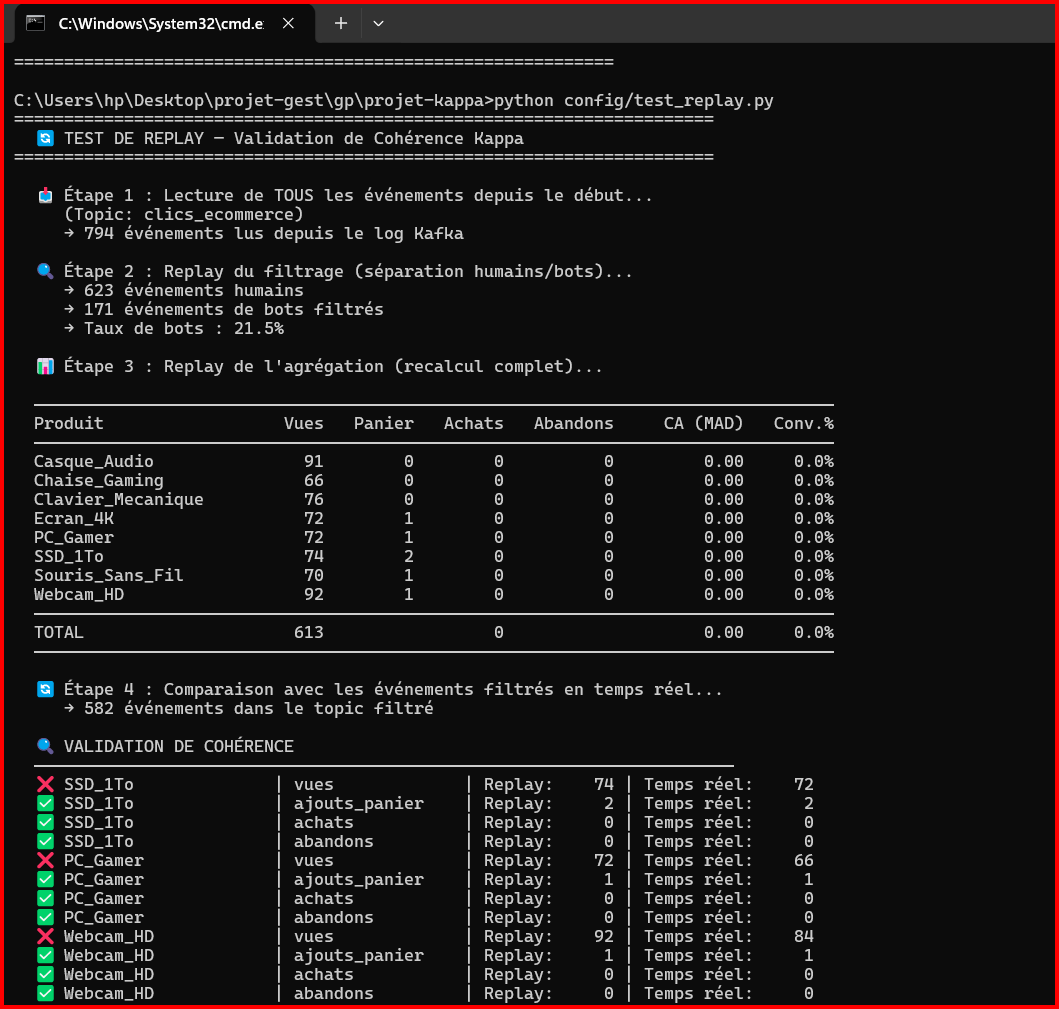
\includegraphics[width=\textwidth]{../screenshots/validation_replay1.png}
    \captionof{figure}{Test de Replay validant la parfaite cohérence avec le traitement temps réel}
\end{borderedfigure}

\section{Scénarios de Replay en Entreprise}

Le mécanisme de replay n'est pas limité à notre cas d'usage. En production, il couvre de nombreux scénarios critiques :

\begin{table}[H]
\centering
\begin{tabularx}{\textwidth}{L{3.5cm} L{4cm} X}
\toprule
\textbf{\color{primarycolor}Scénario} &
\textbf{\color{primarycolor}Action} &
\textbf{\color{primarycolor}Bénéfice} \\
\midrule
Bug dans la formule & Corriger le code, rejouer & Résultats corrigés sans perte de données \\
\addlinespace[0.1cm]
Nouveau KPI demandé & Ajouter la métrique, rejouer & KPI historique disponible immédiatement \\
\addlinespace[0.1cm]
Audit de données & Rejouer et comparer & Preuve de cohérence et traçabilité \\
\addlinespace[0.1cm]
Migration de système & Rejouer sur le nouveau système & Validation de la migration \\
\addlinespace[0.1cm]
Test de charge & Rejouer $N$ fois plus vite & Mesure de performance et scalabilité \\
\bottomrule
\end{tabularx}
\caption{Scénarios de replay en environnement professionnel}
\end{table}

\section{Limites et Bonnes Pratiques}

\begin{table}[H]
\centering
\begin{tabularx}{\textwidth}{L{3cm} X X}
\toprule
\textbf{\color{primarycolor}Limite} &
\textbf{\color{primarycolor}Impact} &
\textbf{\color{primarycolor}Solution} \\
\midrule
Espace disque & Plus de rétention = plus de stockage & Compression des messages Kafka \\
\addlinespace[0.1cm]
Temps de replay & Rejouer 7 jours d'événements prend du temps & Replay partiel (depuis un offset précis) \\
\addlinespace[0.1cm]
Coût & Stockage cloud potentiellement coûteux & Politique de rétention adaptée au besoin métier \\
\bottomrule
\end{tabularx}
\caption{Limites de la rétention et solutions}
\end{table}

\begin{infobox}
    \textbf{Bonne pratique :} Définir la rétention en fonction du besoin métier. 7 jours suffisent pour notre cas d'usage e-commerce, mais un système bancaire pourrait nécessiter 90 jours ou plus.
\end{infobox}
